\documentclass[a4paper,10pt]{article}
\usepackage[utf8]{inputenc}
\makeatletter
\def\input@path{ {/home/jeremy/Documents/} }
\input{macros}
\makeatother

%opening
\title{}
\author{}

\begin{document}

\maketitle

\section{Setup}
With the group data $\delta = [-1/2,1/2], q = [1/4,1/4]$ we get the following image of $D_\zeta$ and $D_\zeta'$. 
\begin{figure}[ht!]
\centering
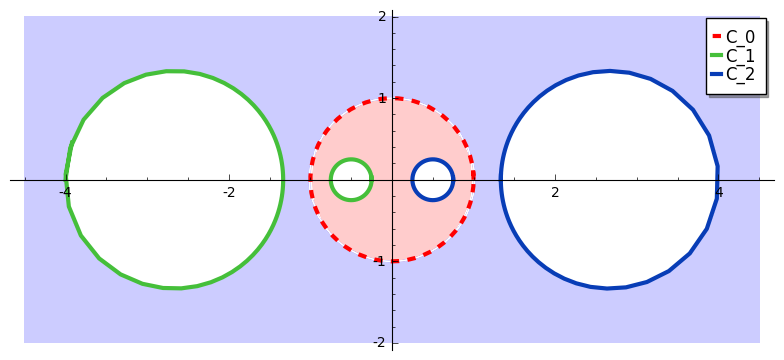
\includegraphics[width=0.7\textwidth]{product_threshold_test-FundamentalDomain.png} 
\end{figure}
The union of the red shaded region and the purple shaded region is the fundamental domain, $F$. 

\section{Results}
All current tests (15/1/31) passed in all cases of \verb+product_threshold+
\begin{table}[h!]
 \centering
 \begin{tabular}{c|c|c|c|c}
  product\_threshold &  build $\omega$ time (s) & slitmap time (s)& abs((5.17)) & approx branch pts \\\hline
  2 & 3.2 & 0.99 & 0.85 & [(-3.549561, -1.002919), (1.003466, 6.763318)] \\ \hline
3 & 0.40 & 1.5 & 2.5 & [(-1.036200, -1.002797), (1.003321, 1.048239)] \\ \hline
4 & 0.72 & 2.2 & 4.1 & [(-1.036062, -1.002788), (1.003332, 1.048425)] \\ \hline
5 & 0.95 & 3.1 & 5.2 & [(-1.035680, -1.002785), (1.003328, 1.047908)] \\ \hline
6 & 1.4 & 4.4 & 5.9 & [(-1.035676, -1.002785), (1.003329, 1.047912)] \\ \hline
7 & 2.0 & 6.4 & 6.3 & [(-1.035669, -1.002785), (1.003329, 1.047903)] \\ \hline
8 & 3.1 & 11. & 6.5 & [(-1.035669, -1.002785), (1.003329, 1.047903)] \\ \hline
9 & 5.5 & 30. & 6.6 & [(-1.035668, -1.002785), (1.003329, 1.047902)] \\ \hline
10 & 13. & 110. & 6.7 & [(-1.035668, -1.002785), (1.003329, 1.047902)] \\ \hline
11 & 37. & 310. & 6.8 & [(-1.035668, -1.002785), (1.003329, 1.047902)] \\ \hline
 \end{tabular}
\end{table}
  
 We get the following figures
\begin{table}[!ht]
 \begin{tabular}{|c|c|c|}
  \hline
  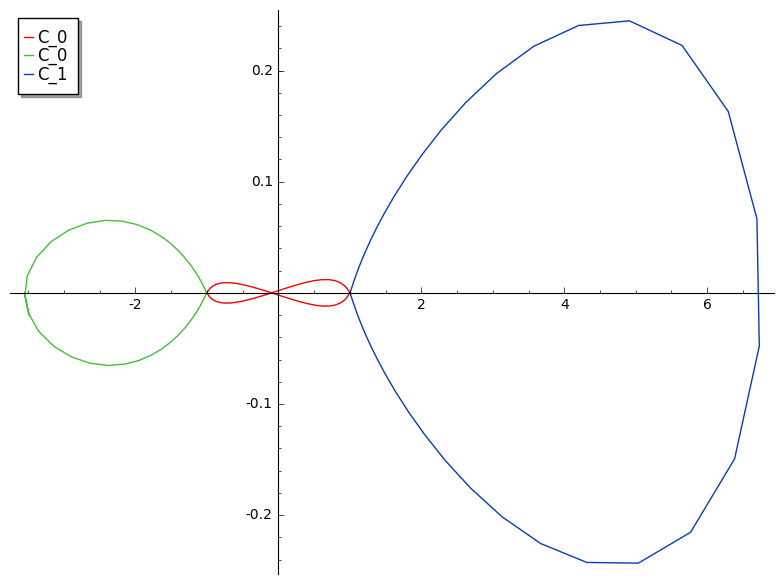
\includegraphics[width=0.3\textwidth]{product_threshold_test1_threshold-2.png} & 
  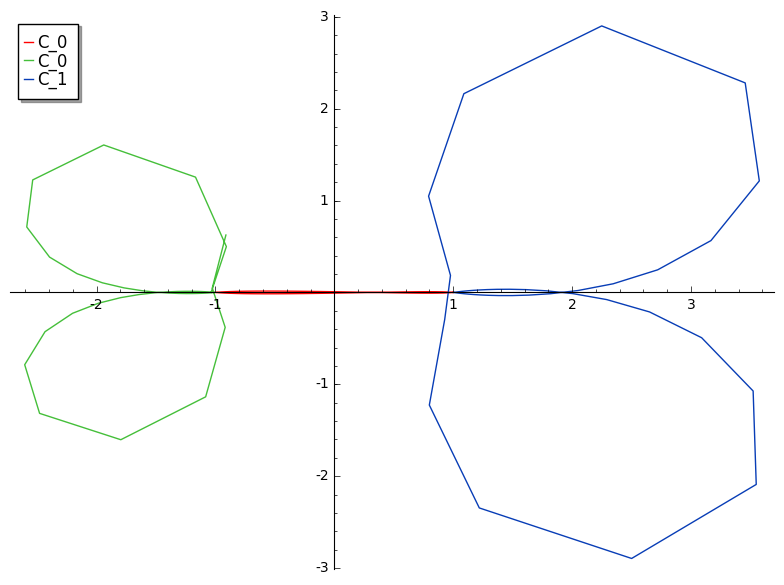
\includegraphics[width=0.3\textwidth]{product_threshold_test1_threshold-3.png} &
  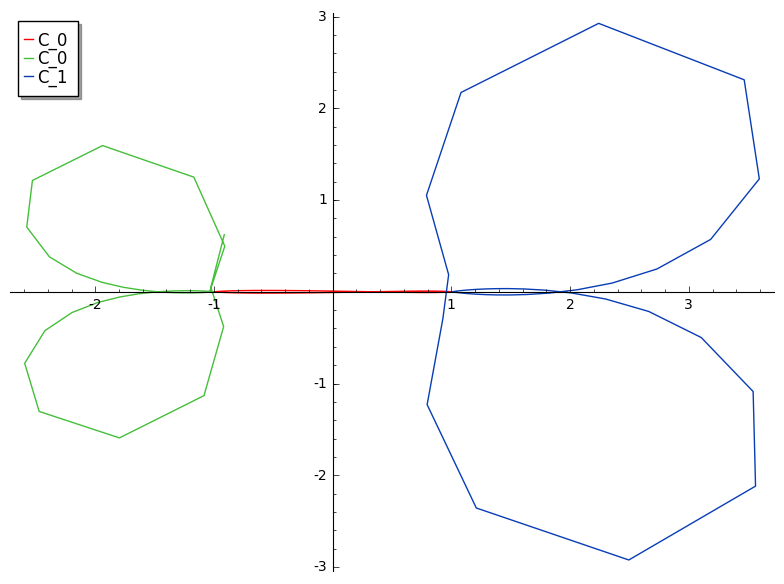
\includegraphics[width=0.3\textwidth]{product_threshold_test1_threshold-4.png} \\\hline
  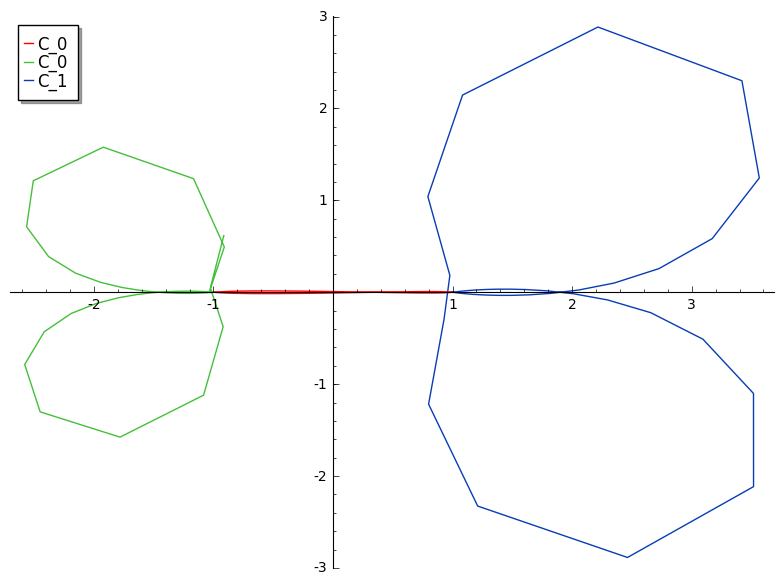
\includegraphics[width=0.3\textwidth]{product_threshold_test1_threshold-5.png} & 
  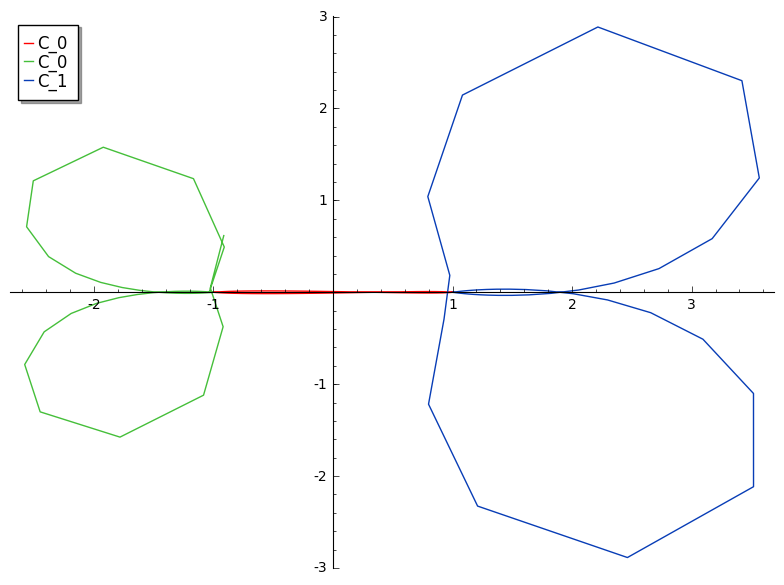
\includegraphics[width=0.3\textwidth]{product_threshold_test1_threshold-6.png} &
  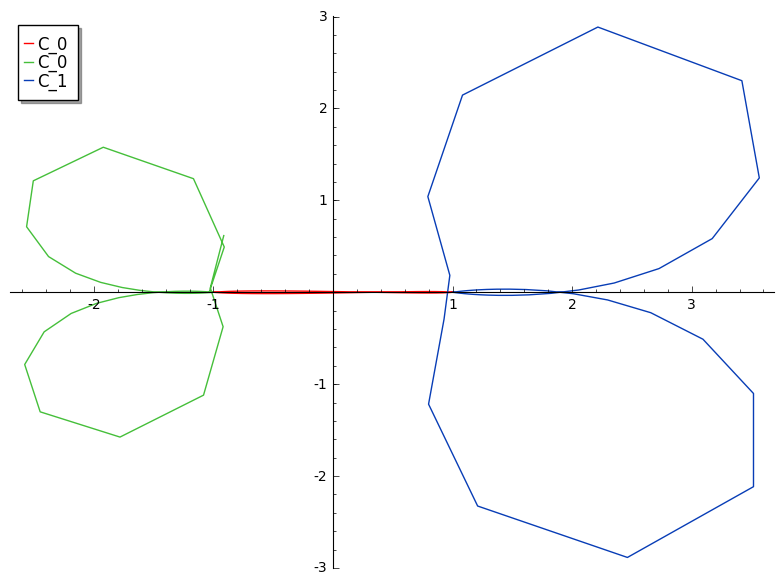
\includegraphics[width=0.3\textwidth]{product_threshold_test1_threshold-7.png} \\\hline
  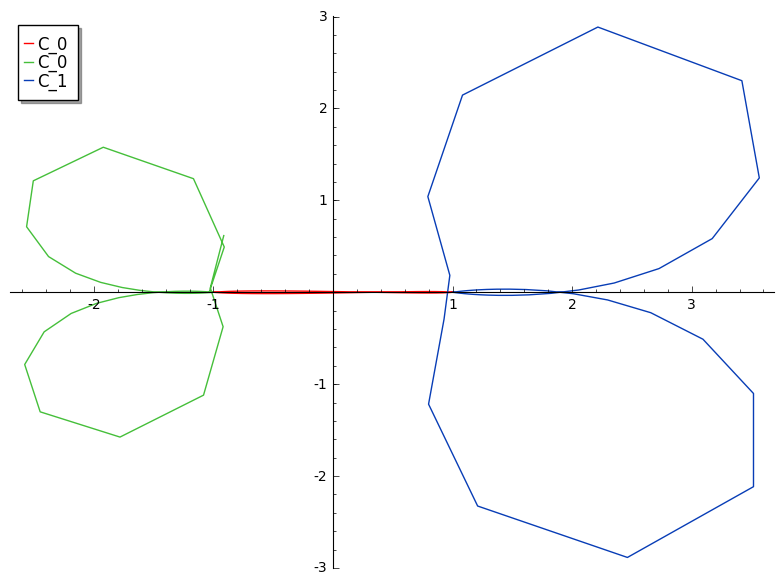
\includegraphics[width=0.3\textwidth]{product_threshold_test1_threshold-8.png} & 
  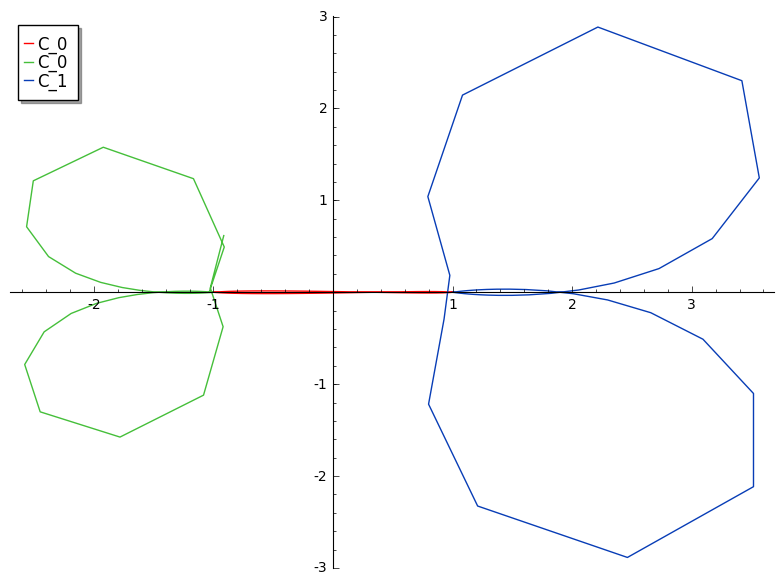
\includegraphics[width=0.3\textwidth]{product_threshold_test1_threshold-9.png} &
  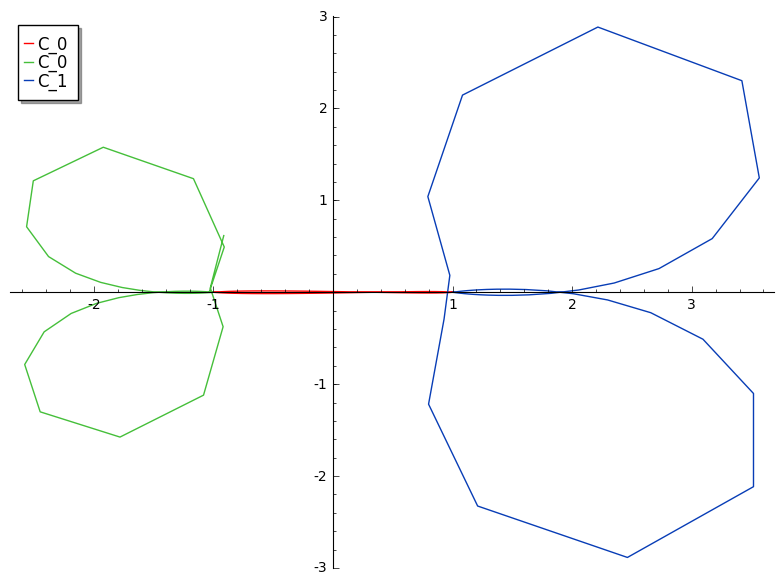
\includegraphics[width=0.3\textwidth]{product_threshold_test1_threshold-10.png} \\\hline
 \end{tabular}
 \caption{For product\_threshold = 2,...,10, left to right top to bottom.}
\end{table}
 
 These figures are clearly showing something bad. The circles should be collapsing to intervals. Look at more detail for product\_threshold = 3 after using the control of product\_threshold = 1 and product\_threshold=2 (which look like I would expect.)
 
 
 \subsection{Results - product\_threshold=1}
 We get the following images:
 \begin{table}[!ht]
 \caption{product\_threshold=1}
 \begin{tabular}{|c|c|c|}
  \hline
  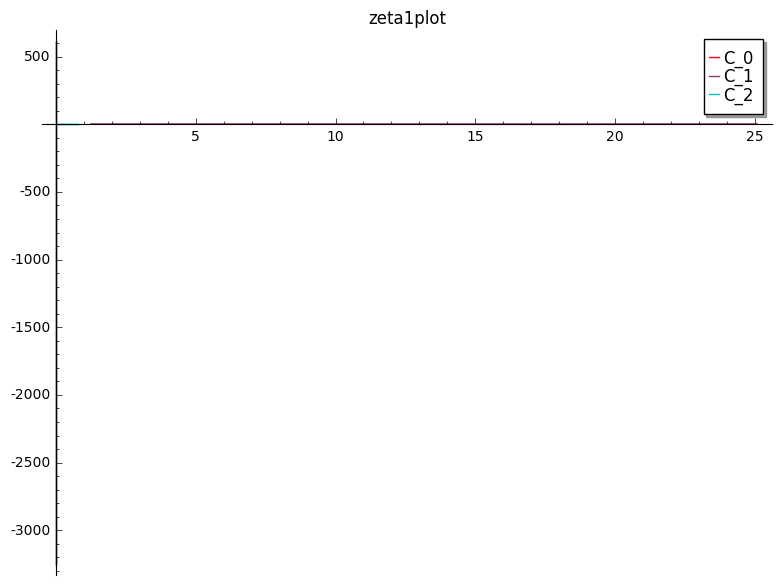
\includegraphics[width=0.3\textwidth]{PT_1_z1.png} &
  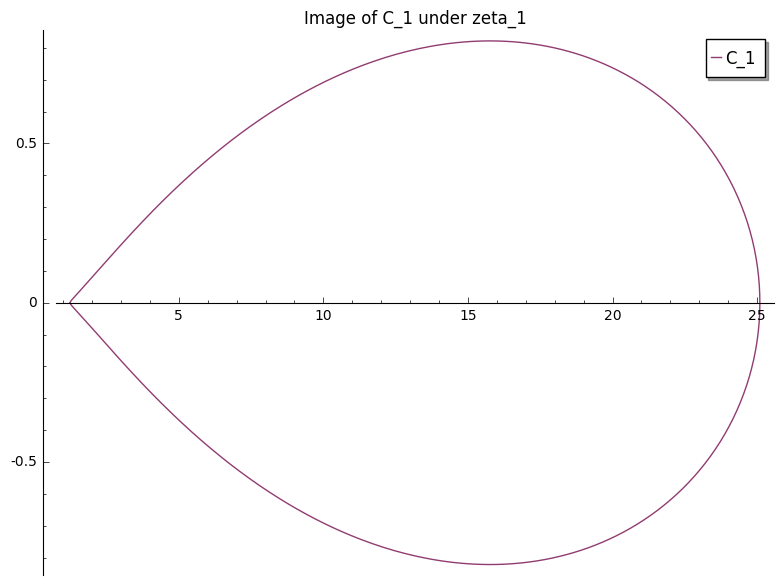
\includegraphics[width=0.3\textwidth]{PT_1_C1z1.png} &
  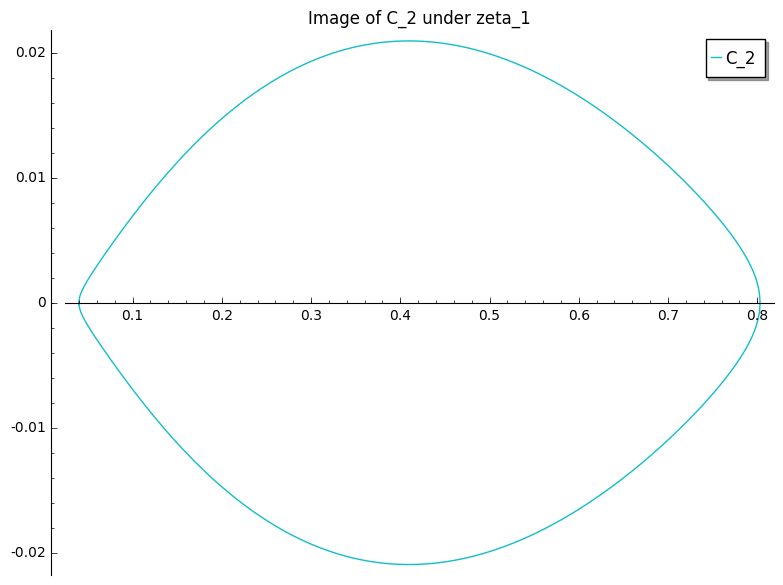
\includegraphics[width=0.3\textwidth]{PT_1_C2z1.png} \\ \hline
  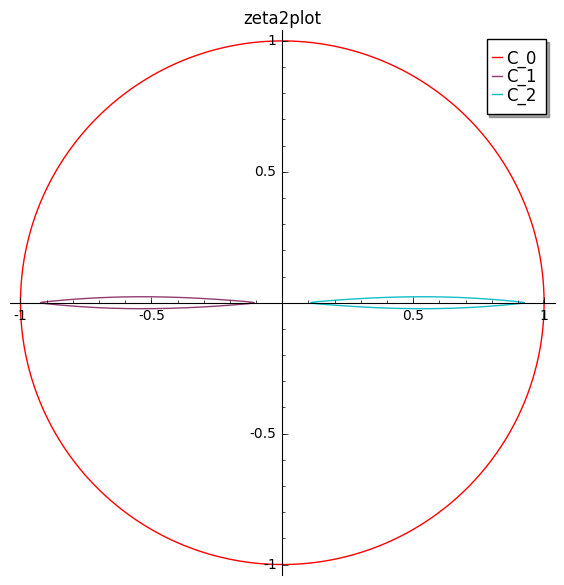
\includegraphics[width=0.3\textwidth]{PT_1_z2.png} &
  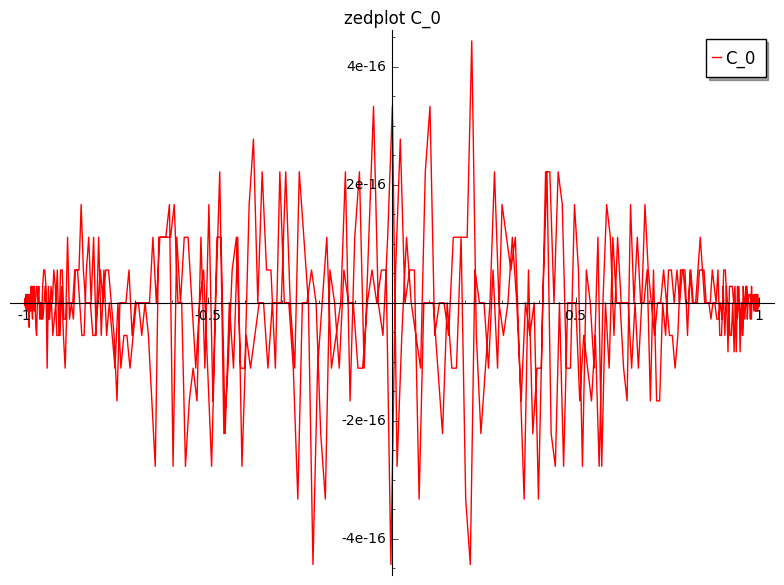
\includegraphics[width=0.3\textwidth]{PT_1_zed_C0.png} &
  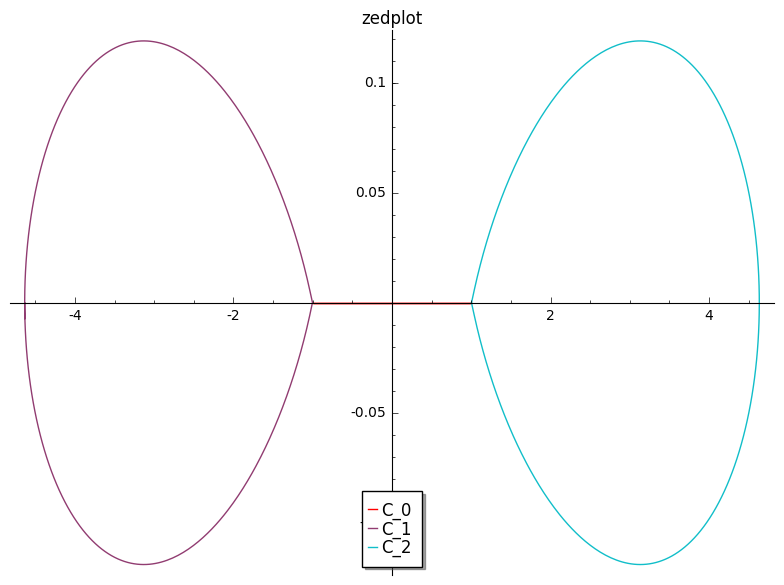
\includegraphics[width=0.3\textwidth]{PT_1_zed.png} \\ \hline
 \end{tabular}
 \end{table}
 
 \subsection{Results - product\_threshold=2}
 We get the following images:
 \begin{table}[!ht]
 \caption{product\_threshold=2}
 \begin{tabular}{|c|c|c|}
  \hline
  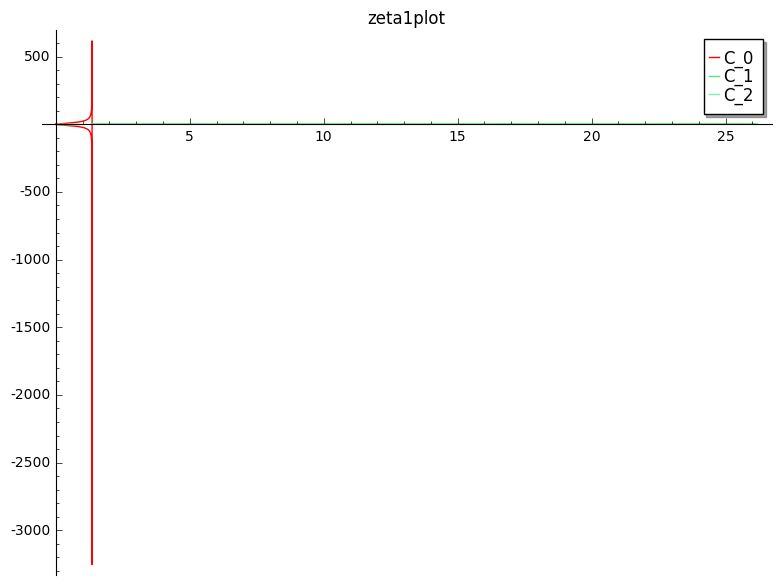
\includegraphics[width=0.3\textwidth]{PT_2_z1.png} &
  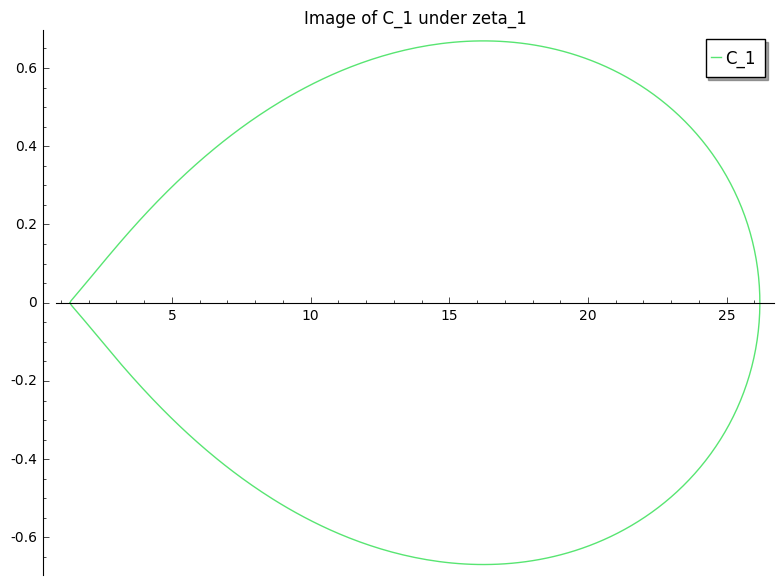
\includegraphics[width=0.3\textwidth]{PT_2_C1z1.png} &
  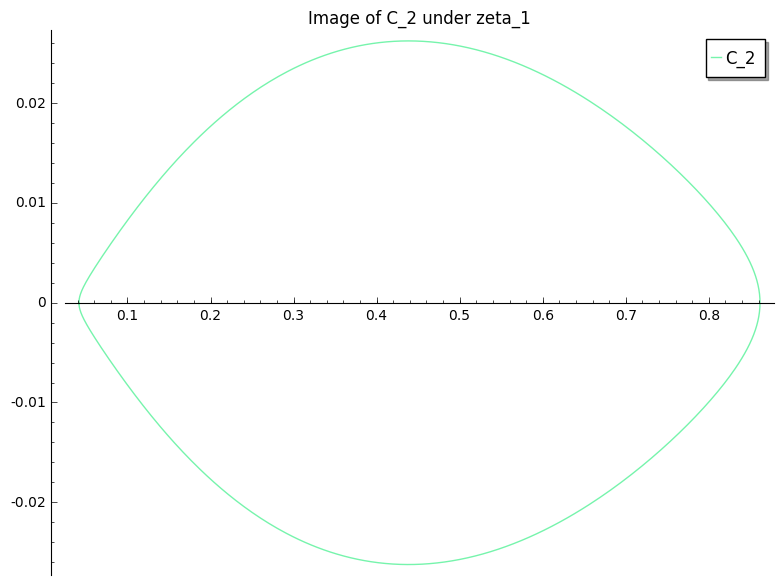
\includegraphics[width=0.3\textwidth]{PT_2_C2z1.png} \\ \hline
  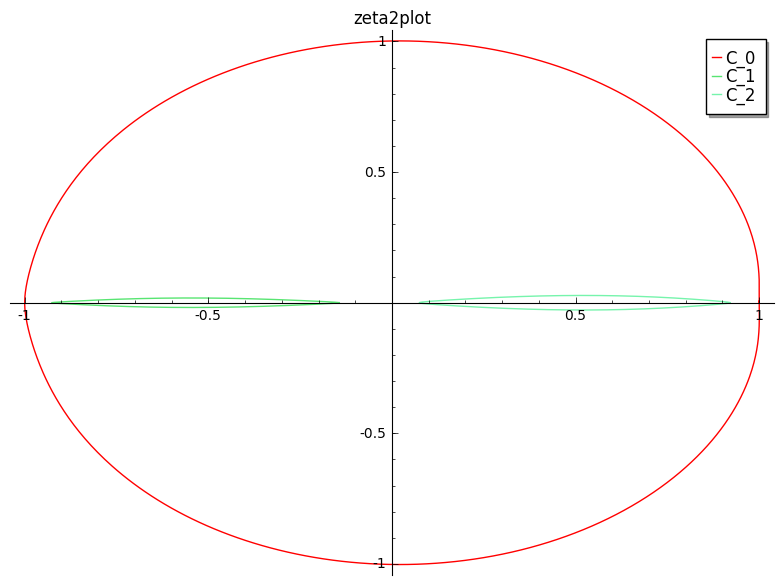
\includegraphics[width=0.3\textwidth]{PT_2_z2.png} &
  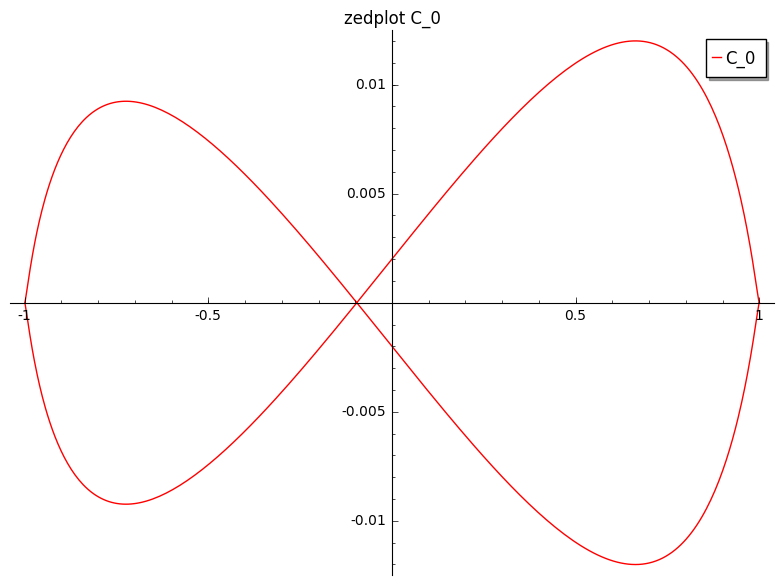
\includegraphics[width=0.3\textwidth]{PT_2_zed_C0.png} &
  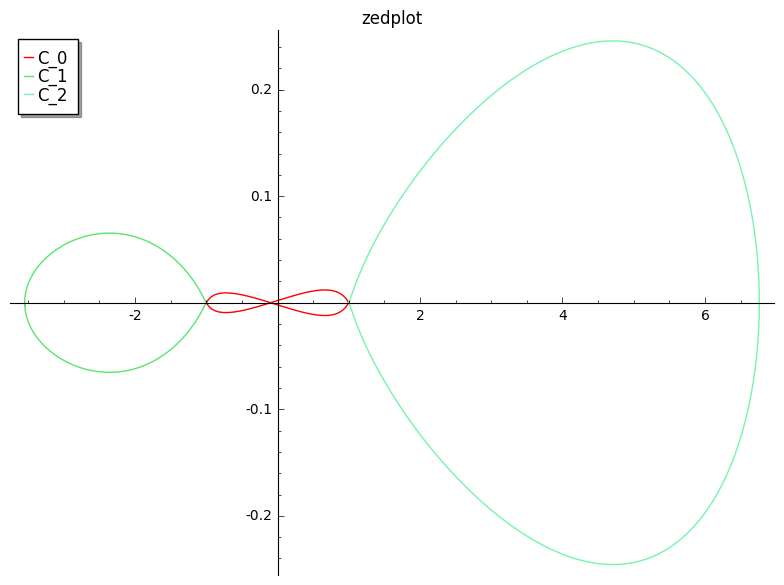
\includegraphics[width=0.3\textwidth]{PT_2_zed.png} \\ \hline
 \end{tabular}
 \end{table}

 \subsection{Results - product\_threshold=3}
 We get the following images:
 \begin{table}[!ht]
 \caption{product\_threshold=3}
 \begin{tabular}{|c|c|c|}
  \hline
  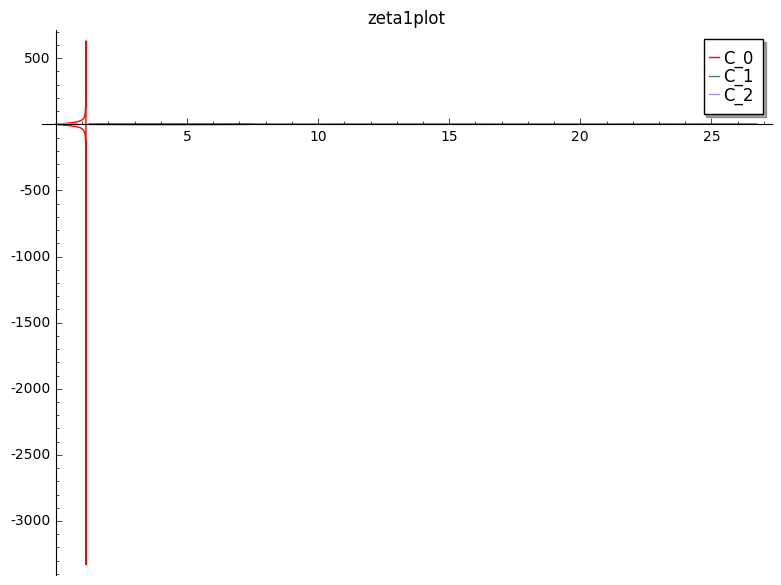
\includegraphics[width=0.3\textwidth]{PT_3_z1.png} &
  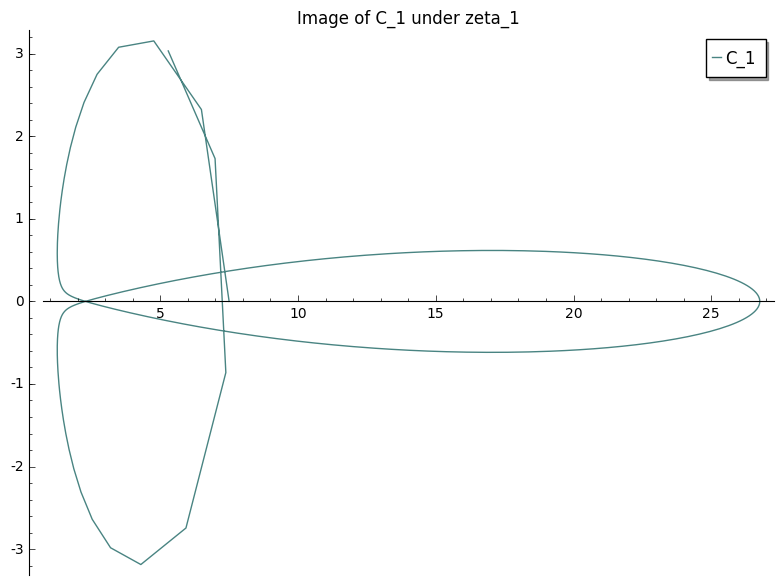
\includegraphics[width=0.3\textwidth]{PT_3_C1z1.png} &
  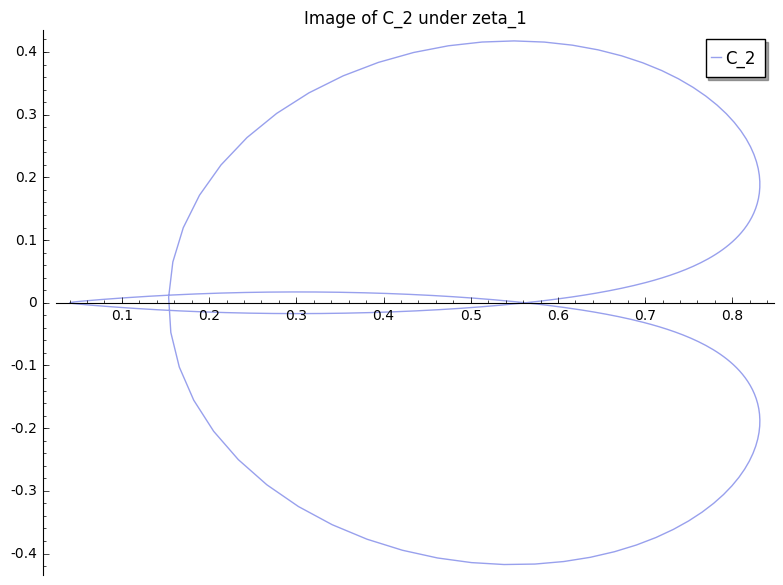
\includegraphics[width=0.3\textwidth]{PT_3_C2z1.png} \\ \hline
  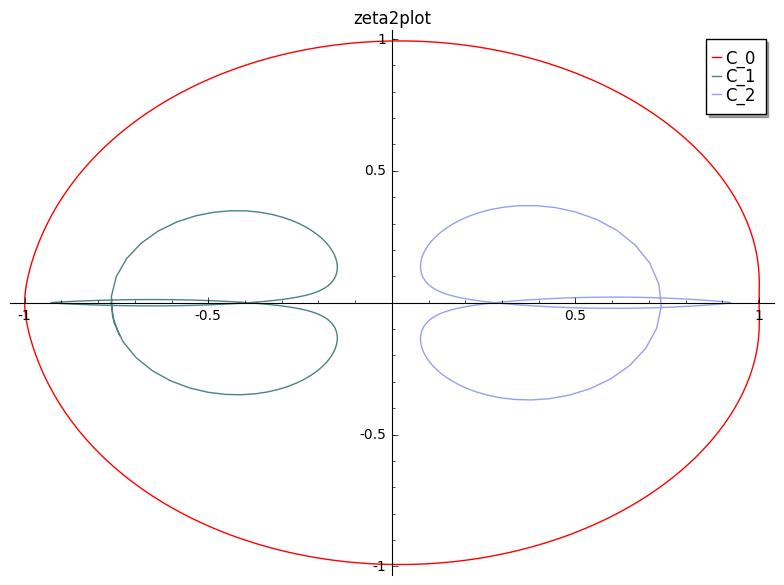
\includegraphics[width=0.3\textwidth]{PT_3_z2.png} &
  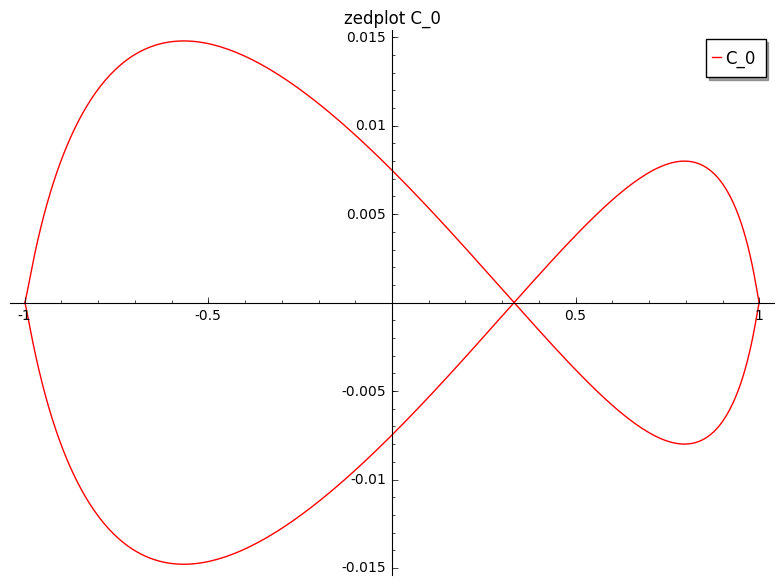
\includegraphics[width=0.3\textwidth]{PT_3_zed_C0.png} &
  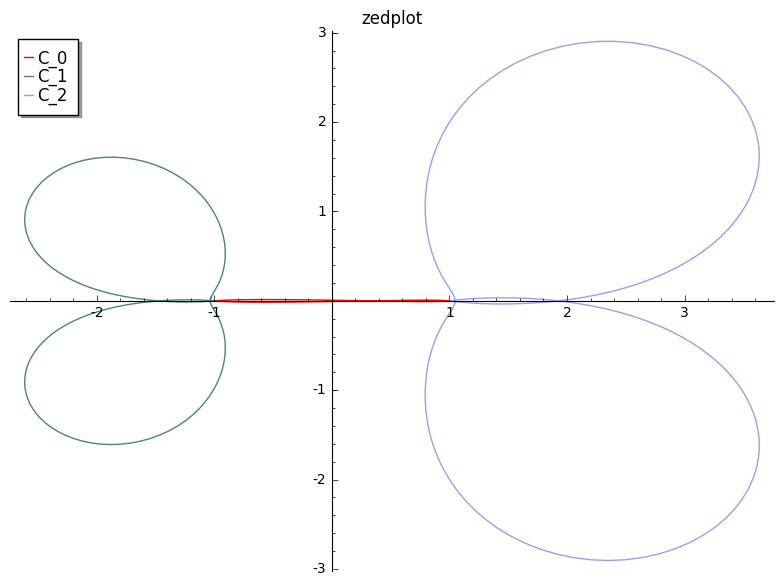
\includegraphics[width=0.3\textwidth]{PT_3_zed.png} \\ \hline
 \end{tabular}
 \end{table}

 Something weird is happening to the $C_j$ under $\zeta_1$, it is blowing up far too much. However the image of $C_0$ is behaving as we expect. 
 
 If we read page 190 of the text, we see that the two relations (5.10) and (5.17) satisfied by the prime function together show that $\zeta_1(\zeta) = \zeta_1(\zeta)$ for $\zeta$ on $C_j$. I.e. each circle $C_j$ should map to the real $\zeta_1$ axis! This should be checked.
 
 \subsubsection{Using only the word $\phi_1^3$}
 We get the following images:
 \begin{table}[!ht]
 \caption{product\_threshold=3, $\phi_1^3$ only}
 \begin{tabular}{|c|c|c|}
  \hline
  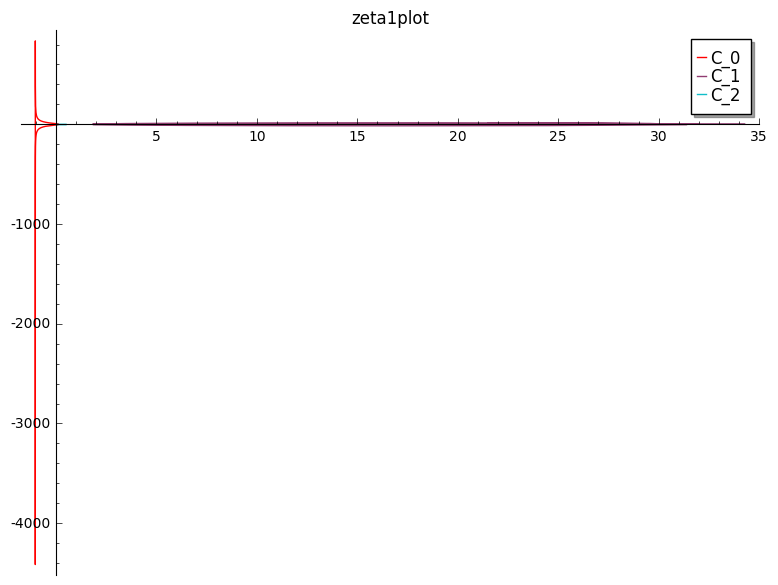
\includegraphics[width=0.3\textwidth]{PT_3_z1_1-3.png} &
  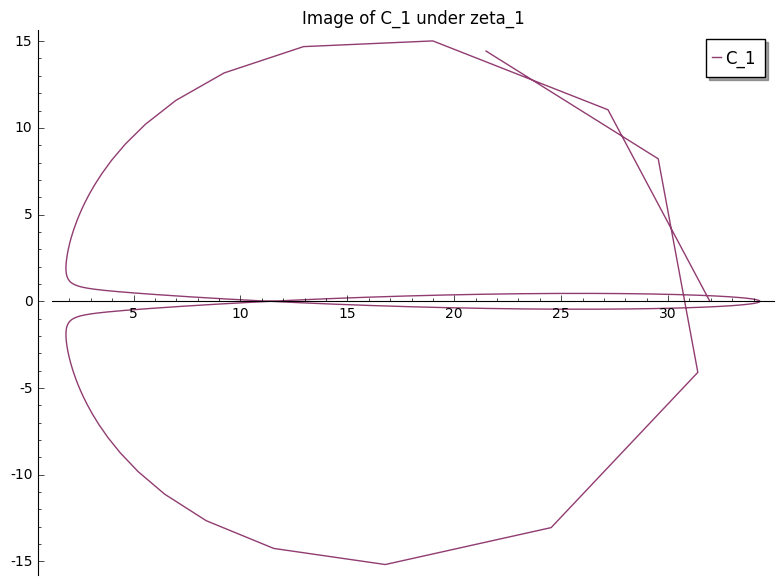
\includegraphics[width=0.3\textwidth]{PT_3_C1z1_1-3.png} &
  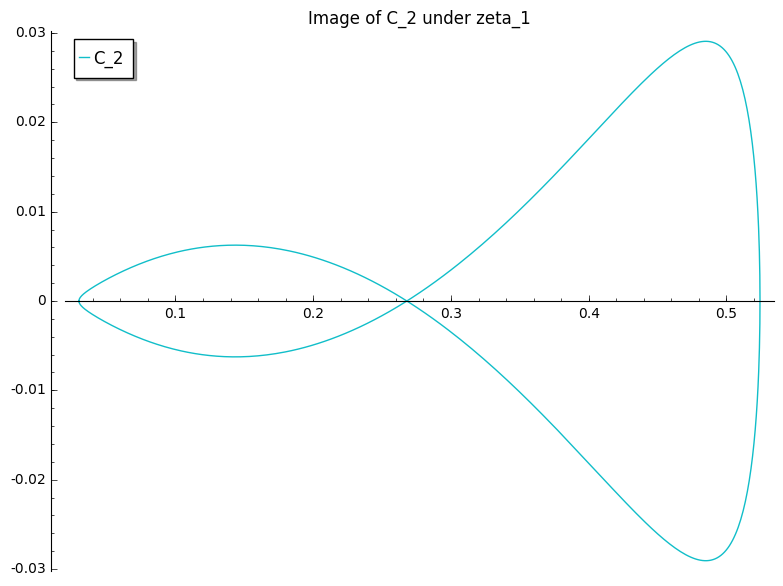
\includegraphics[width=0.3\textwidth]{PT_3_C2z1_1-3.png} \\ \hline
  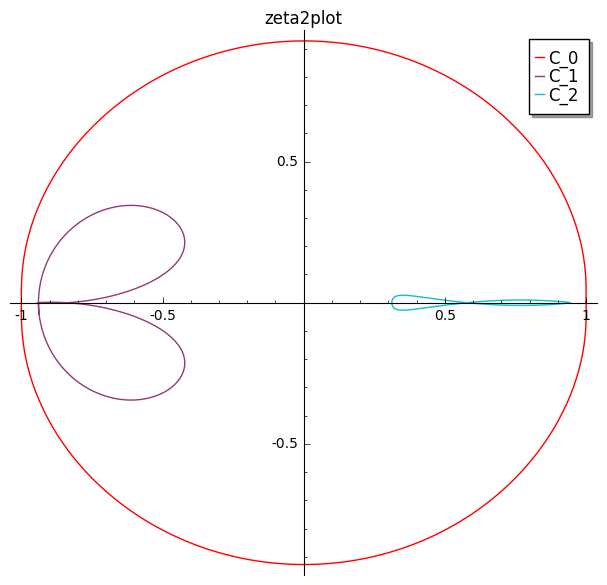
\includegraphics[width=0.3\textwidth]{PT_3_z2_1-3.png} &
  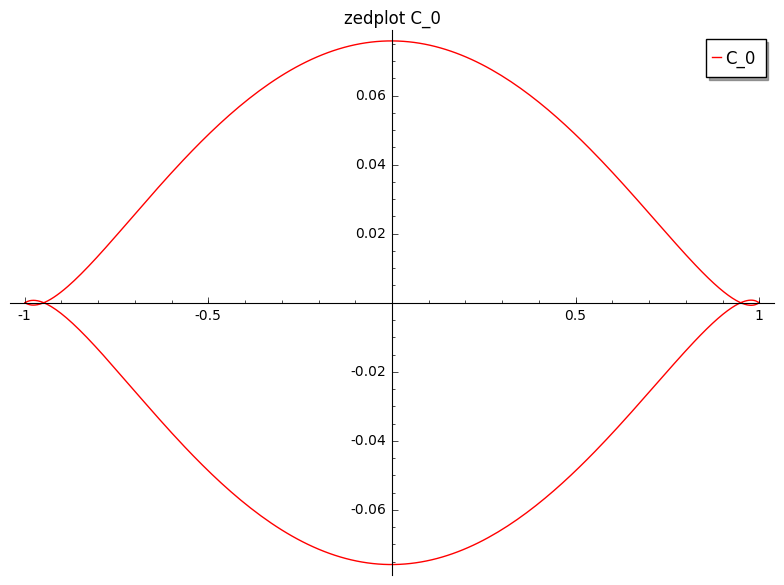
\includegraphics[width=0.3\textwidth]{PT_3_zed_C0_1-3.png} &
  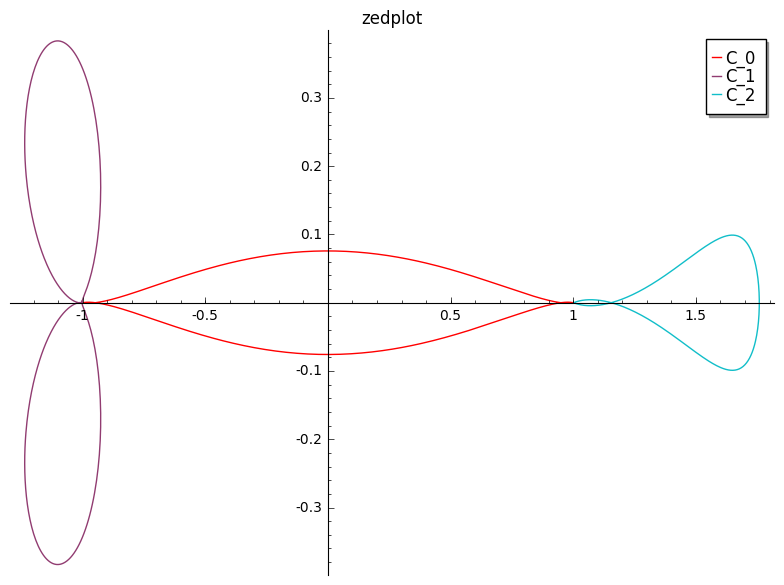
\includegraphics[width=0.3\textwidth]{PT_3_zed_1-3.png} \\ \hline
 \end{tabular}
 \end{table}
 
 \subsubsection{Using only the word $\phi_1^2*\phi_2$}
 We get the following images:
 \begin{table}[!ht]
 \caption{product\_threshold=3, $\phi_1^2*\phi_2$ only}
 \begin{tabular}{|c|c|c|}
  \hline
  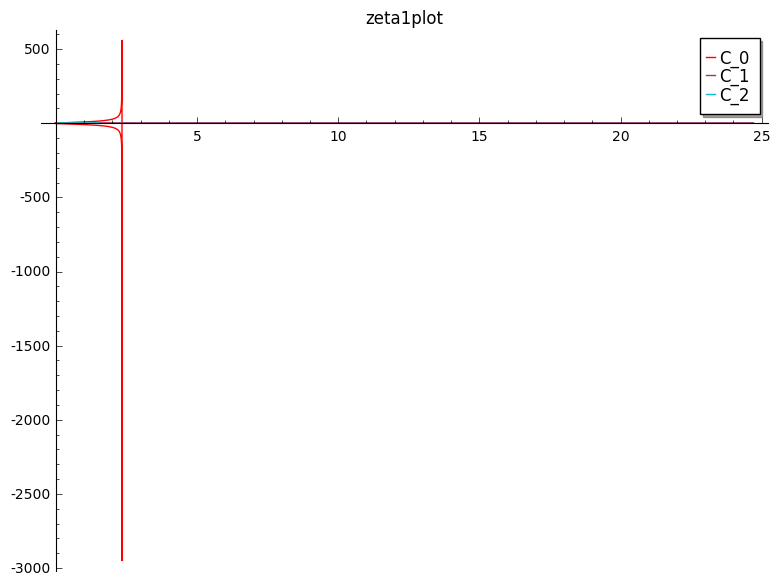
\includegraphics[width=0.3\textwidth]{PT_3_z1_1-2_2-1.png} &
  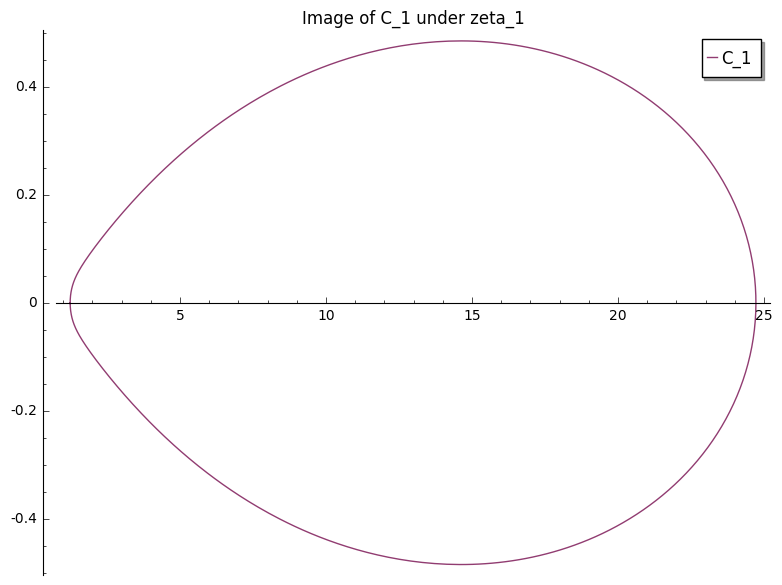
\includegraphics[width=0.3\textwidth]{PT_3_C1z1_1-2_2-1.png} &
  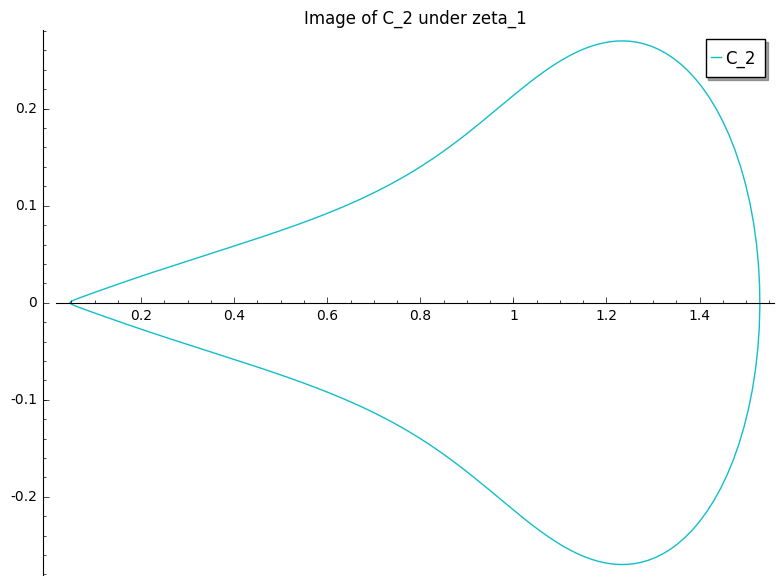
\includegraphics[width=0.3\textwidth]{PT_3_C2z1_1-2_2-1.png} \\ \hline
  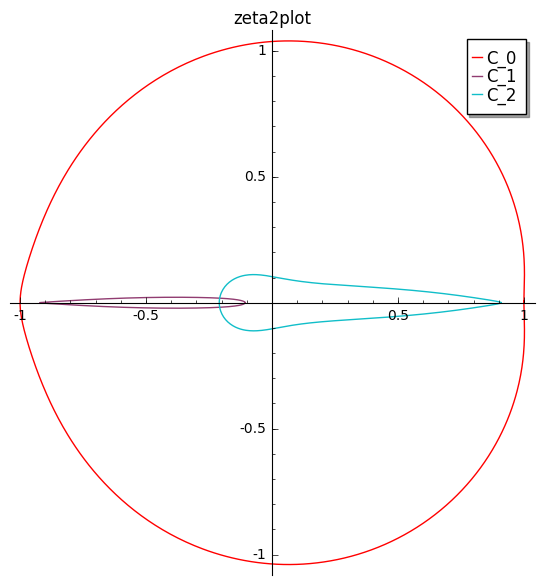
\includegraphics[width=0.3\textwidth]{PT_3_z2_1-2_2-1.png} &
  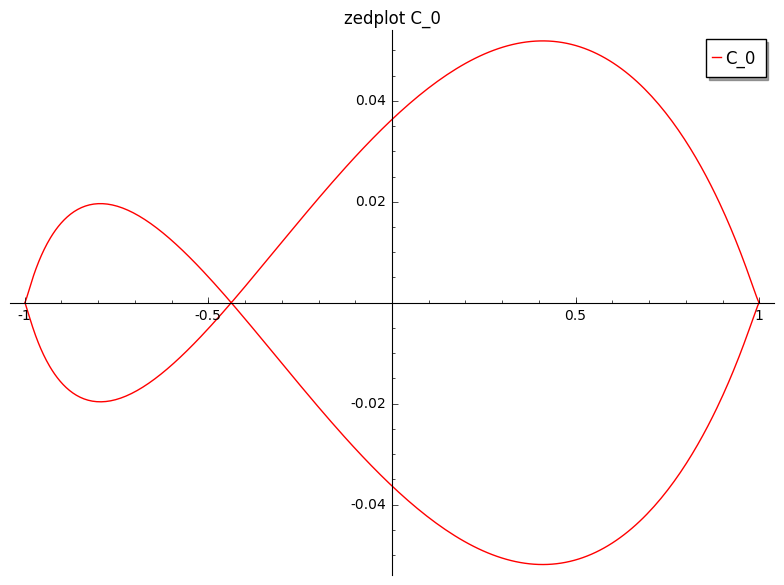
\includegraphics[width=0.3\textwidth]{PT_3_zed_C0_1-2_2-1.png} &
  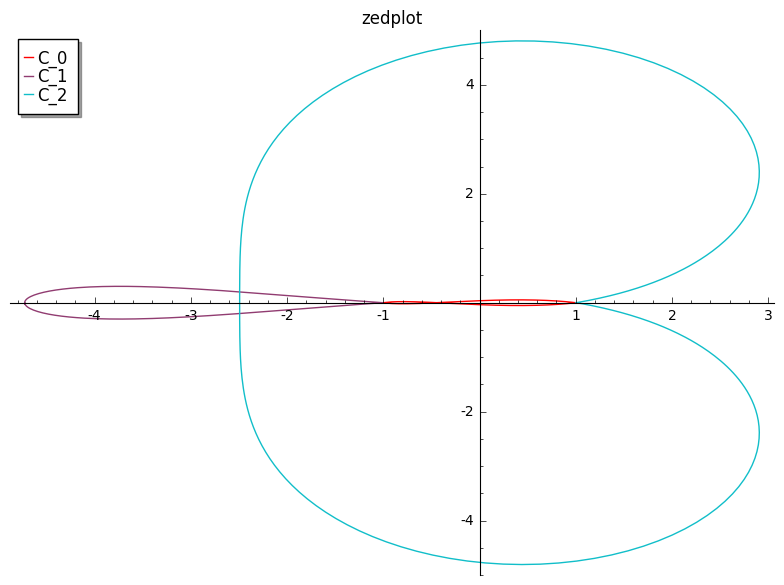
\includegraphics[width=0.3\textwidth]{PT_3_zed_1-2_2-1.png} \\ \hline
 \end{tabular}
 \end{table}
 
 \subsubsection{Using only the word $\phi_1*\phi_2*\phi_1$}
 We get the following images:
 \begin{table}[!ht]
 \caption{product\_threshold=3, $\phi_1*\phi_2*\phi_1$ only}
 \begin{tabular}{|c|c|c|}
  \hline
  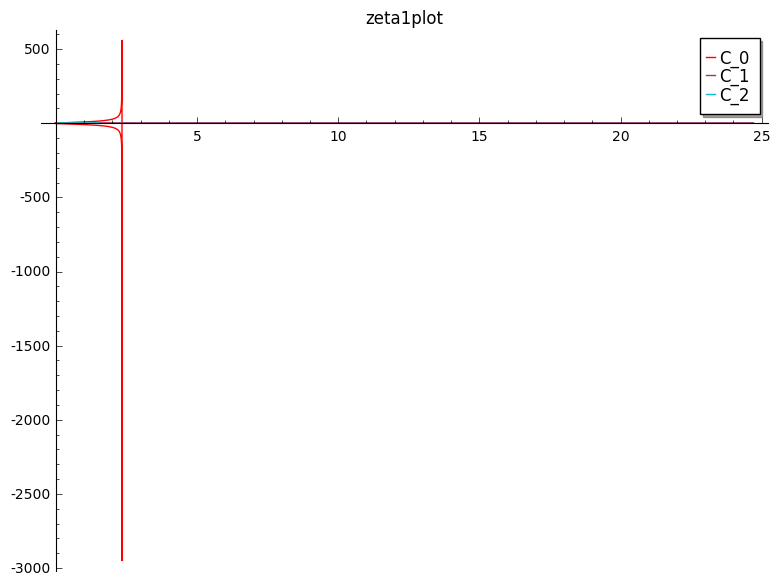
\includegraphics[width=0.3\textwidth]{PT_3_z1_1-1_2-1_1-1.png} &
  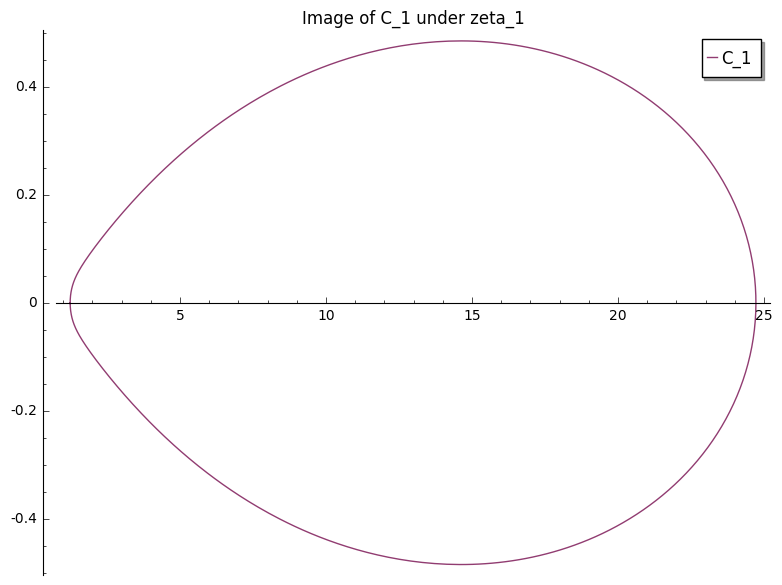
\includegraphics[width=0.3\textwidth]{PT_3_C1z1_1-1_2-1_1-1.png} &
  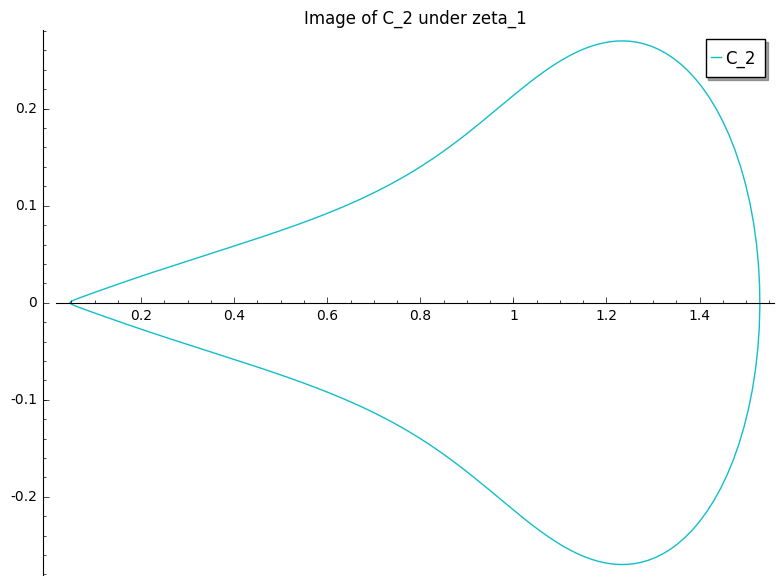
\includegraphics[width=0.3\textwidth]{PT_3_C2z1_1-1_2-1_1-1.png} \\ \hline
  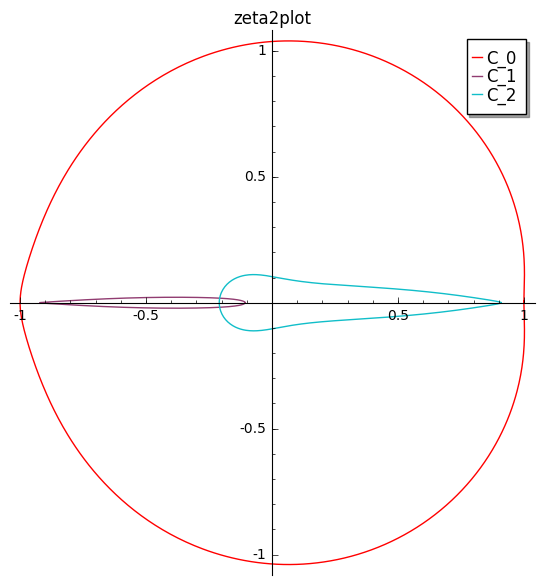
\includegraphics[width=0.3\textwidth]{PT_3_z2_1-1_2-1_1-1.png} &
  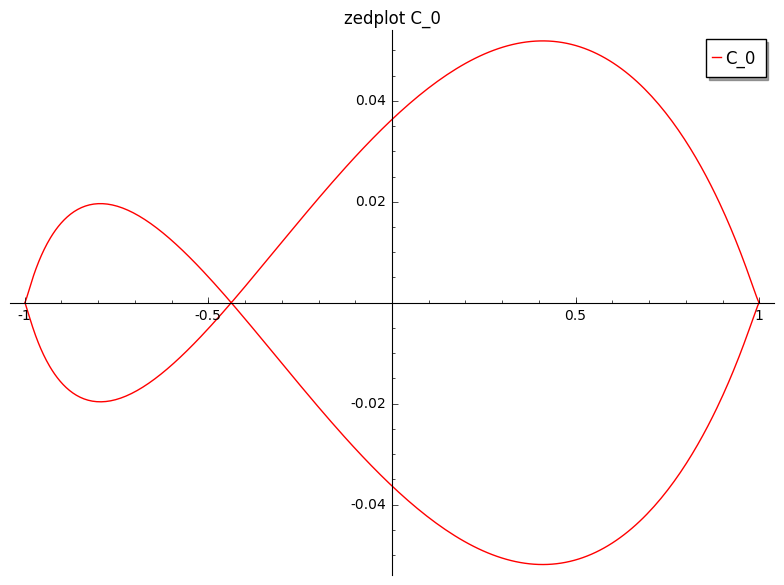
\includegraphics[width=0.3\textwidth]{PT_3_zed_C0_1-1_2-1_1-1.png} &
  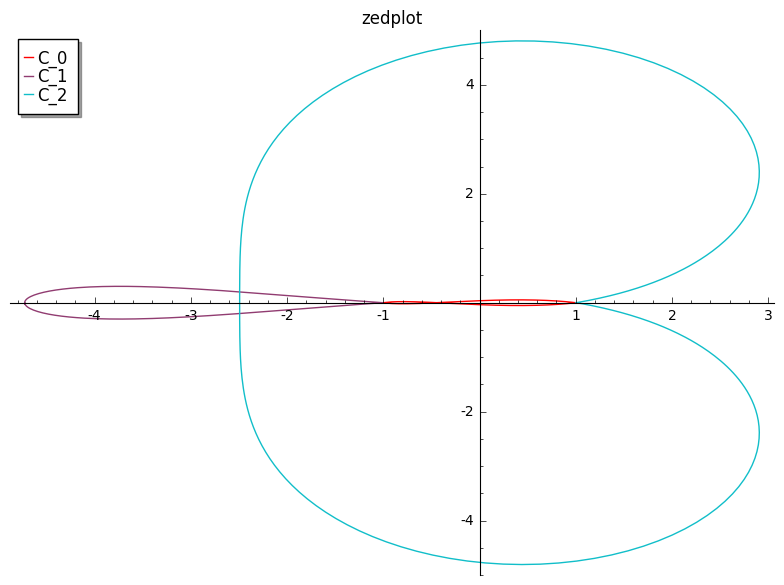
\includegraphics[width=0.3\textwidth]{PT_3_zed_1-1_2-1_1-1.png} \\ \hline
 \end{tabular}
 \end{table}
 Notice that this is the exact same as above! Because the functions are all abelian!

 \subsubsection{Using only the word $\phi_1*\phi_2^2$}
 We get the following images:
 \begin{table}[!ht]
 \caption{product\_threshold=3, $\phi_1*\phi_2^2$ only}
 \begin{tabular}{|c|c|c|}
  \hline
  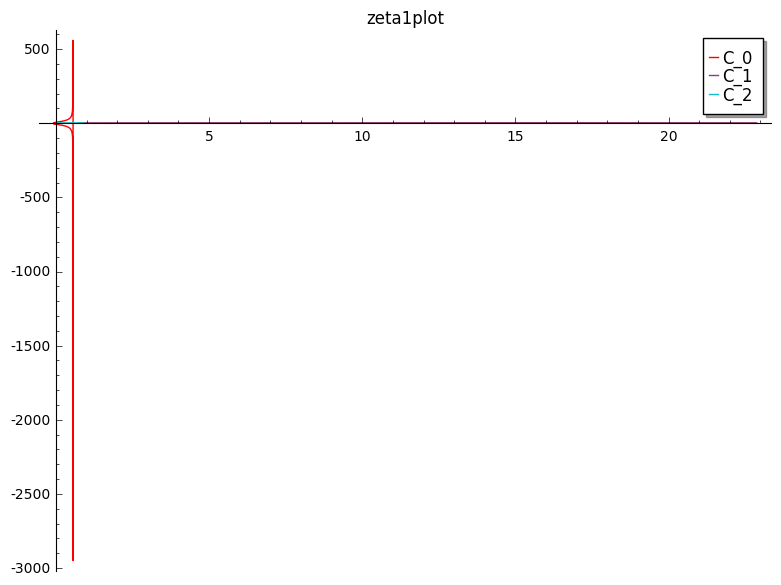
\includegraphics[width=0.3\textwidth]{PT_3_z1_1-1_2-2.png} &
  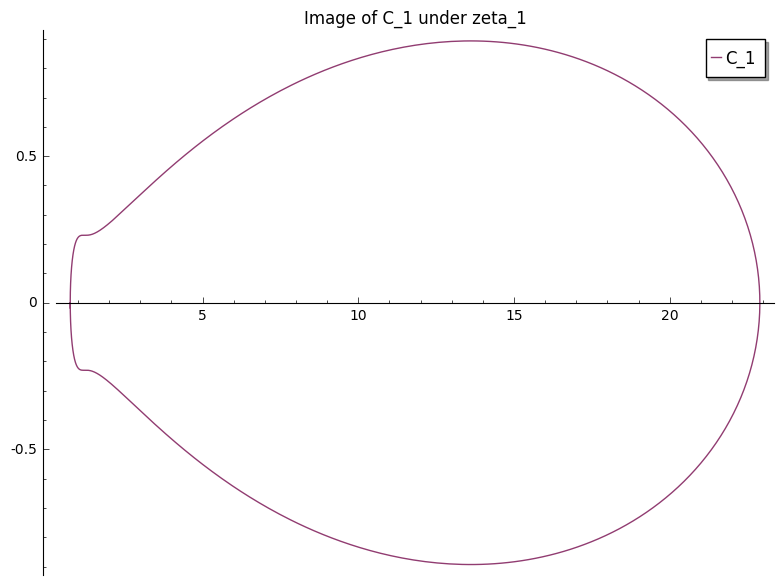
\includegraphics[width=0.3\textwidth]{PT_3_C1z1_1-1_2-2.png} &
  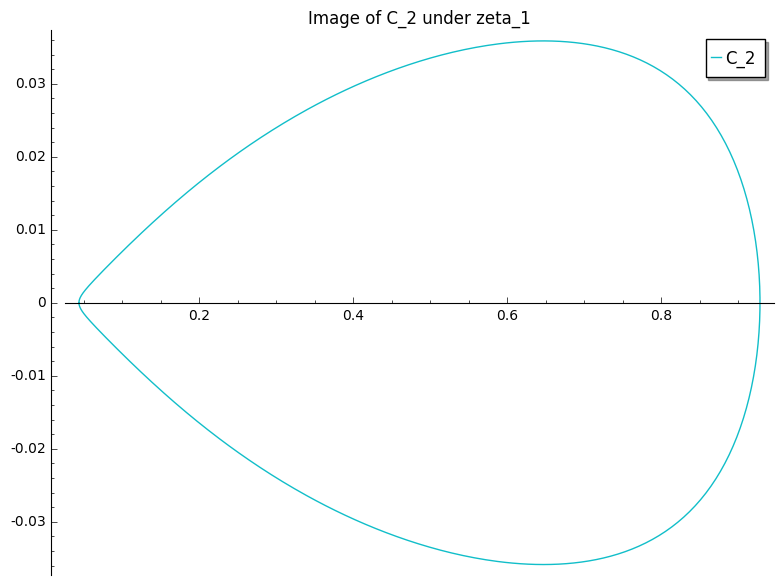
\includegraphics[width=0.3\textwidth]{PT_3_C2z1_1-1_2-2.png} \\ \hline
  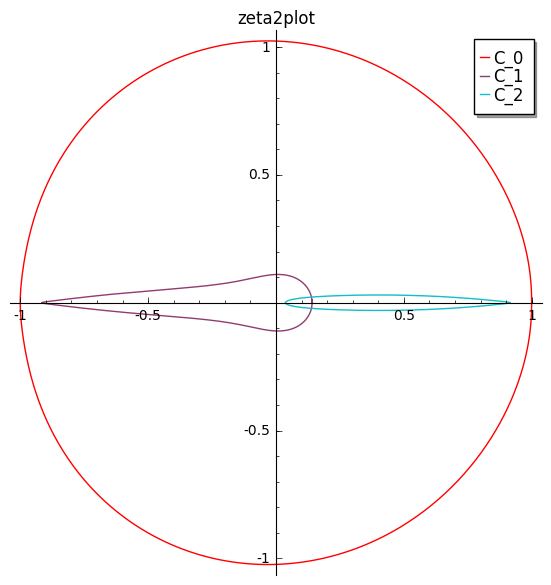
\includegraphics[width=0.3\textwidth]{PT_3_z2_1-1_2-2.png} &
  \includegraphics[width=0.3\textwidth]{PT_3_zed_C0_1-1_2-2.png} &
  \includegraphics[width=0.3\textwidth]{PT_3_zed_1-1_2-2.png} \\ \hline
 \end{tabular}
 \end{table}
 
 \subsubsection{Using only the word $\phi_2*\phi_1^2$}
 This looks exactly the same as the word $\phi_1^2\phi_2$ for example, so the plots are omitted. Further plots are also omitted!
 

 \section{Something is strange here. Shouldn't these maps be symmetric? Why would they not be? Plot just $\phi_1$ and $\phi_2$}
 \subsection{$\phi_1$}
 The code gives: \verb?phi_i = 1/8*z/(z+2)-1/2? and
 \begin{verbatim}
  omegap=(8*gamma - z/(z + 2) + 4)*(8*z - gamma/(gamma + 2) + 4)/
	                           ((8*gamma - gamma/(gamma + 2) + 4)*(8*z - z/(z + 2) + 4)).
 \end{verbatim}
 
 We get the following images:
 \begin{table}[!ht]
 \caption{product\_threshold=1, $\phi_1$ only}
 \begin{tabular}{|c|c|c|}
  \hline
  \includegraphics[width=0.3\textwidth]{PT_1_z1_1.png} &
  \includegraphics[width=0.3\textwidth]{PT_1_C1z1_1.png} &
  \includegraphics[width=0.3\textwidth]{PT_1_C2z1_1.png} \\ \hline
  \includegraphics[width=0.3\textwidth]{PT_1_z2_1.png} &
  \includegraphics[width=0.3\textwidth]{PT_1_zed_C0_1.png} &
  \includegraphics[width=0.3\textwidth]{PT_1_zed_1.png} \\ \hline
 \end{tabular}
 \end{table}

 \subsection{$\phi_2$}
 The code gives: \verb?phi_i = -1/8*z/(z-2)+1/2? and
 \begin{verbatim}
  omegap=(8*gamma + z/(z - 2) - 4)*(8*z + gamma/(gamma - 2) - 4)
                         /((8*gamma + gamma/(gamma - 2) - 4)*(8*z + z/(z - 2) - 4)).
 \end{verbatim}
 
 We get the following images:
 \begin{table}[!ht]
 \caption{product\_threshold=1, $\phi_2$ only}
 \begin{tabular}{|c|c|c|}
  \hline
  \includegraphics[width=0.3\textwidth]{PT_1_z1_2.png} &
  \includegraphics[width=0.3\textwidth]{PT_1_C1z1_2.png} &
  \includegraphics[width=0.3\textwidth]{PT_1_C2z1_2.png} \\ \hline
  \includegraphics[width=0.3\textwidth]{PT_1_z2_2.png} &
  \includegraphics[width=0.3\textwidth]{PT_1_zed_C0_2.png} &
  \includegraphics[width=0.3\textwidth]{PT_1_zed_2.png} \\ \hline
 \end{tabular}
 \end{table}






\end{document}
